\chapter[Capítulo 3. Metodolog\'ia.]{Metodologia}
\pagestyle


\section[Descripción General del Sistema]{Descripción General del Sistema}

El modelo conceptual del sistema, está compuesto por varios subsistemas o bloques escalables, independientes y que se pueden comunican entre s\'i, mediante un un intermediario que se encarga de coordinar los datos entre los distintos bloques. El sistema general se podr\'ia dividir en tres segmentos principales, por un lado el subsistema central \textit{la sonda}, de mayor complejidad que se encarga de recepci\'on y transmisi\'on de datos y nexo con los otros subsistemas, ejecuta el muestreo con los sensores, almacena en una base local los datos, la \textit{estacion remota}, la sala de monitoreo donde se puede visualizar los datos recibido de la sonda y realizar configuraciones de muestreo, los subsistemas menos complejos se denominar perif\'ericos, son bloques auxiliares escalables en medida que sean necesarios, y de esa forma aumentar las funcionalidades del sistema, en el presente TFG de desarrollaron e implementaron los perif\'ericos que ayuden para el muestreo a multiniveles como ser perif\'ericos de \textit{batimetr\'ia}, para conocer la profundidad del lugar de muestreo y perif\'erico de \textit{gr\'ua} que le otorga a la sonda la posibilidad de desplazamiento vertical para pueda tomar muestras a multiniveles y el perif\'erico \textit{ASV}, provee la ubicaci\'on georeferenciada del punto de muestreo y otorga a la sonda la posibilidad de desplazamiento horizontal sobre toda la superficie a ser analizada. Los modos de operaci\'on pueden ser autom\'aticos, donde ejecuta un algoritmo en sincron\'ia con el ASV o manual donde el usuario desde la estaci\'on remota puede configurar los par\'ametros que requiera.  
El diagrama de funcionamiento del sistema se pude apreciar en la Figura \ref{fig:3.1}.


\begin{figure}[H]
    \centering
    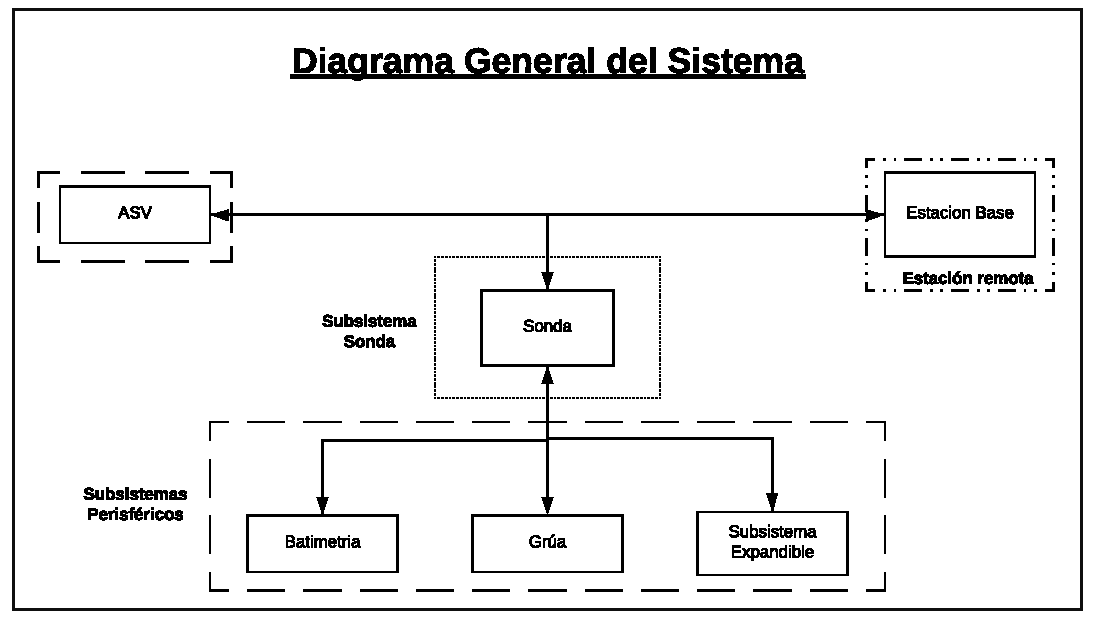
\includegraphics[width=150mm, height=70mm]{Imagenes/2021/img31.pdf}
    \caption[Diagrama General del Sistema]{Diagrama General del Sistema. \textbf{Fuente:} Elaboración Propia.}
    \label{fig:3.1}
\end{figure}



\subsubsection{Sonda}
\section[Bloque de Control]{Bloque de Control}
Este bloque es el encargado de realizar el procesamiento de los datos recibidos a través de los sensores y la configuración de parámetros adquirida por la Interfaz de Usuario.

\begin{itemize}
    \item \textbf{Hardware:}
    En la Figura \ref{fig:4.4} se observa la placa de desarrollo low cost escogida para el presente proyecto, la Raspberry Pi 3 model B desarrollado por la fundación Raspberry Pi. La misma cuenta con un procesador multimedia Broadcom BCM2835 system-on-chip (SoC).
    \newline
    \hfill
    La CPU Contiene un ARM1176JZFS, con unidad de coma flotante, que funciona a 700Mhz y es capaz de soportar overclock a 1GHZ en modo “TURBO” que hace que el SoC de más rendimiento sin reducir el tiempo de vida de la placa y sin perder la garantía. 
    La memoria RAM es de 512MB de SDRAM (en su modelo B), en un único módulo, el cual, funciona a 400Mhz en su modo normal y alcanzando los 600Mhz en su versión “TURBO”.
    La  Raspberry Pi no tiene un disco duro tradicional, para ello dispone de un lector para memorias SD, un sistema de almacenamiento en estado sólido. El arranque del sistema se hará desde la propia tarjeta SD, con lo que, debido a que tiene que albergar todo el sistema operativo, es necesario que la tarjeta sea de al menos 2 GB de capacidad para almacenar todos los archivos requeridos.
    La placa carece de botón de encendido y apagado, con lo que la energía le llega mediante un conector microUSB estándar de 5V. El consumo de la placa es de 700mA, (3,5W).
    La Raspberry Pi, está diseñada para ejecutar el sistema operativo GNU/Linux y la version mas extendido es el Raspberry Pi OS .
    \begin{figure}[t]
        \centering
        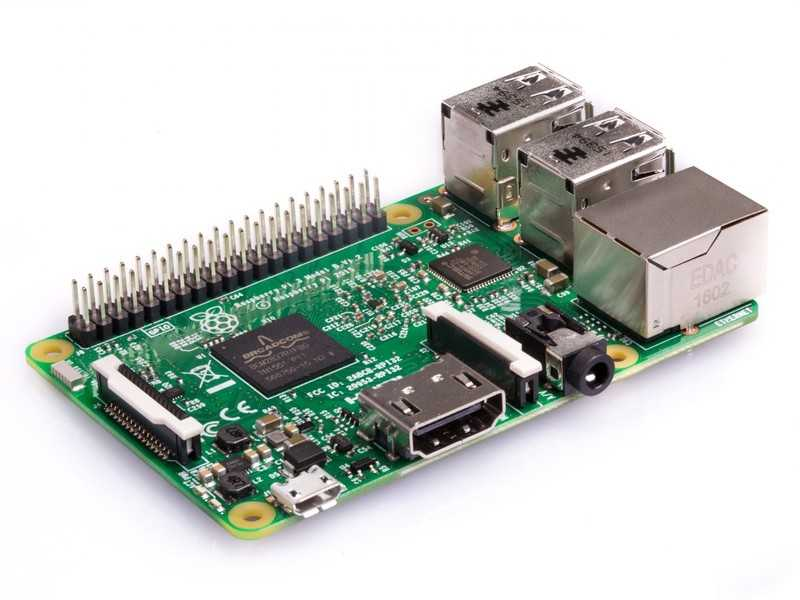
\includegraphics[width=100mm, height=70mm]{Imagenes/2021/imag35.jpg}
        \caption[Placa Raspberry Pi 3 model B]{Placa Raspberry Pi 3 model B.\textbf{Fuente:} Página Web del Fabricante.}
        \label{fig:4.4}
    \end{figure}


    Se optó por este controlador por sus prestaciones prestaciones t/'ecnicas, suficientes para las tareas a ser ejecutadas, con un almacenamiento externa de 32 Gb con una memoria tipo microSD de alto rendimiento, sus dimensiones reducidas eran acorde a los requerimientos necesarios y por tener un gran soporte y comunidad activa en linea.
 
    En la Tabla \ref{tab:carac_rasp} se detallan las principales características técnicas de la Raspberry Pi 3 model B.
 
 \begin{table}[t]
      \protect\caption[Características Técnicas. Raspberry Pi 3 model B]{Características Técnicas. Raspberry Pi 3 model B.  \label{tab:carac_rasp}}
    
     \centering
     \begin{tabular}{|l|c|}
        \hline
           Sistema Operativo & Raspberry Pi OS\\
          \hline
          Juego de Instrucciones & RISC 64 bits\\
          \hline
          Procesador & RQuad Core 1.2GHz Broadcom BCM2837\\
          \hline
          RAM  & 1 GB\\
          \hline
          Bluetooth &  4.2 Low Energy (BLE)\\
          \hline
          Puertos USB 2.0 & 4\\
          \hline
          GPIO& 40\\
          \hline
          UART& 2\\
          \hline
          I2C& 4\\
          \hline
          Stero/Video & 1\\
          \hline
          HDMI & 1\\
          \hline
          CSI(RPI Camera) & 1\\
          \hline
          DSI(RSP Touchscreen display) & 1\\
          \hline
          Dimensiones & 85.60 mm x 53.98 mm\\
          \hline
          Peso & 50 g\\
          \hline
          Consumo energ\'etico & 4 W\\
          \hline
          Alimentaci\'on & 5 V\\
          \hline
        
     \end{tabular}
     \vspace{5mm}
     \newline
     \hfill \textbf{Fuente:} Elaboración Propia. Información recopilada de \cite{rasp}
\end{table}
    Por otra parte, para eliminar la necesidad de cableado, multiplexación y aislamiento eléctrico en la lectura de los sensores, se optó por la utilización de la placa open source Tentacle Shield para arduino de Whitebox labs, la cual se muestra en la Figura \ref{fig:4.5}.
\begin{figure}[t]
    \centering
    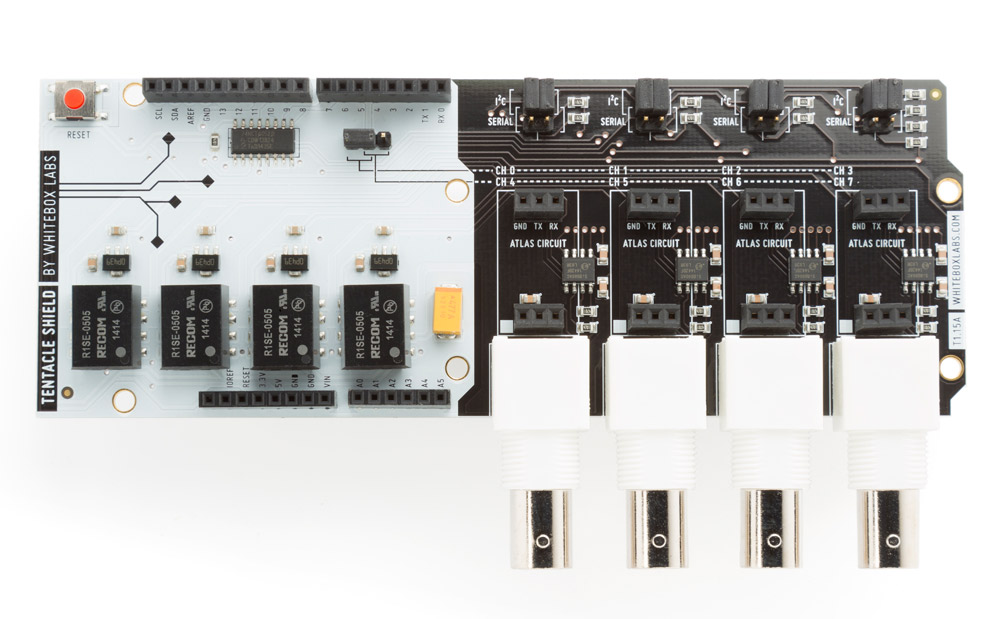
\includegraphics[width=100mm, height=100mm]{Imagenes/2021/imag26.jpg}
    \caption[Placa Tentacle para Arduino]{Placa Tentacle para Arduino. \textbf{Fuente:} Página web del Fabricante}
    \label{fig:4.5}
\end{figure}

    Es una forma pr\'actica y fácil de leer múltiples sensores de la empresa Atlas Scientific, la placa puede alojar hasta 4 dispositivos EZO de Atlas Scientific para medir pH(Potencial de Hidrógeno), Oxígeno Disuelto(DO por sus siglas en inglés), conductividad eléctrica(CE), Temperatura(T), Potencial de Reducción de Oxidación(ORP por sus siglas en inglés)

    \textbf{Aislamiento:}
    Los circuitos de medición y las líneas de comunicación aislados individualmente evitan el ruido y los bucles de tierra para obtener mediciones precisas incluso en sistemas de bucle cerrado.Los sensores no interferirán entre sí y la mayoría del ruido eléctrico exterior que puede interferir con las lecturas se reducirá.

    \item \textbf{Software:}El software de control fue desarrollado en el lenguaje de programación Python. Este es un lenguaje interpretado multiparadigma, soporta programación orientada a objetos, imperativa y funcional.
    Python ya viene instalado en el sistema operativo Raspberry Pi OS para Raspberry Pi.Tiene la ventaja de poder utilizar los pines GPIO de la placa de desarrollo para conectar el mundo digital con el mundo físico mediante la programación, facilitando de esta manera el control de la lectura de los distintos sensores y el accionamiento de los actuadores utilizados.
    
    El administrador de Base de Datos utilizado fue Sqlite3, es un sistema de gestión de base de datos ampliamente difundido en el mundo de la programación de aplicaciones móviles.
    La utilización de este gestor fue debido a su gran portabilidad y su capacidad  de gestionar bases de datos de hasta 2 terabyte de tamaño.
    En la Tabla \ref{tab:caract_sqlite} se muestran las características más relevantes de la Base de Datos Sqlite.

    \begin{table}[H]
    \protect\caption[Características del Gestor de Base de Datos SQLITE]{Características del Gestor de Base de Datos SQLITE.\label{tab:caract_sqlite}}
        \centering
        \begin{tabular}{|l|l|}
            \hline
            Soporte & Múltiples tablas,\textit{triggers} y vistas   \\
            \hline
             Lectura y Escritura& \multicolumn{1}{|l|}{\begin{tabular}[c]{@{}l@{}}  Directamente sobre archivos que se encuentran en el disco \\ duro.\end{tabular}} 
             \\
             \hline
             Formato & 
             \multicolumn{1}{|l|}{\begin{tabular}[c]{@{}l@{}}  Multiplataforma. Puede ser utilizado en sistemas de 32 bits \\ o 64 bits.\end{tabular}} 
           \\
             \hline
             Operaciones &\multicolumn{1}{|l|}{\begin{tabular}[c]{@{}l@{}} Realiza operaciones de manera más eficiente y rápido que  \\ MySql y PostgreSQL.\end{tabular}} 
            \\
             \hline
             Interfaz API &\multicolumn{1}{|l|}{\begin{tabular}[c]{@{}l@{}}Opera con diversas Interfaces API lo que permite trabajar  \\con C++, PHP, Python, Groovy, etc.\end{tabular}} 
            \\
             \hline
             Dependencias Externas & No\\
             \hline
             Librerías & Cuentan con acceso para muchos lenguajes de programación.\\
             \hline
             UDF & Soporta funciones SQL definidas por el usuario.\\
             \hline
             Código Fuente & Dominio público y documentación extensa.\\
             \hline
        
        \end{tabular}
        \vspace{5mm}
        \newline
        \hfill \textbf{Fuente: }Pagina Web del desarrollador.\cite{sqlite}
        
    \end{table}
    
\end{itemize}

\section[Interfaz de Sensores]{Interfaz de Sensores}
Es el bloque donde se adquiere toda la información respecto caracteristicas f\'isico - qu\'imica del recurso h\'idrica, para su posterior procesamiento, almacenamiento y transmici\'on a base remoto.

\subsection{Sensor de pH}
En la Figura \ref{fig:4.8} se puede apreciar el sensor de pH por el que se optó fabricado por la empresa Atlas Scientfic.
    \begin{figure}[t]
    \centering
	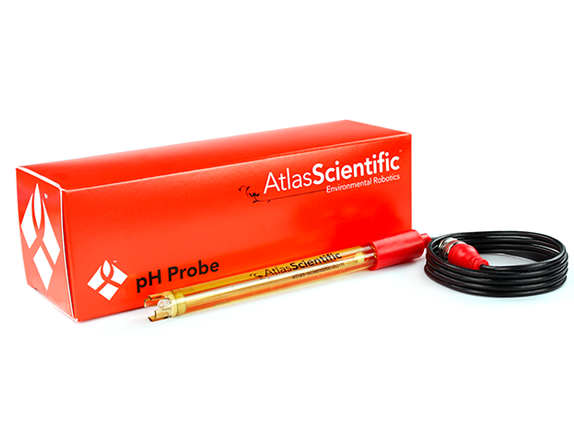
\includegraphics[width=150mm, height=90mm]{Imagenes/2021/imag23.png}%\textwidth%
	\caption[Sonda de pH de la empresa Atlas Scientific]{Sonda de pH de la empresa Atlas Scientific. \textbf{Fuente:} Página Web del fabricante.}
	\label{fig:4.8}
    \end{figure}
Los criterios para la selección de este sensor fueron, su simplicidad de uso gracias a su extensa documentación y soporte por parte del fabricante, su popularidad en el ámbito de la automatización y control de calidad de agua para varios tipos de usos y su integración dentro de la placa de desarrollo sin necesidad de cableados externos y compatible con el módulo EZO pH Circuit que se muestra en la Figura \ref{fig:4.9}
\newline
\hfill
    \begin{figure}[H]
    \centering
	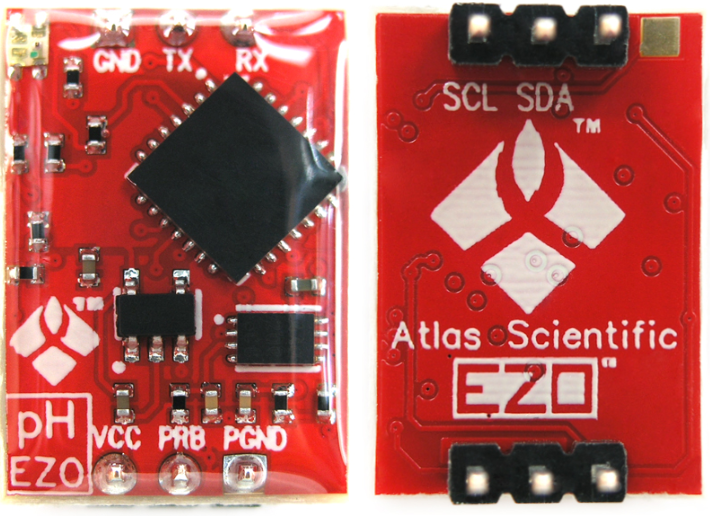
\includegraphics[width=70mm, height=60mm]{Imagenes/2021/imag27.png}%\textwidth%
	\caption[EZO pH Circuit]{EZO pH Circuit.\textbf{Fuente:} Pagina Web del Fabricante.}
	\label{fig:4.9}
    \end{figure}
El módulo es un dispositivo bastante sensible, y ésta sensibilidad es lo que le da una excelente precisión. Significa que es capaz de leer microvoltajes que están presentes en el agua de fuentes no naturales como bombas, válvulas de solenoide u otras sondas o sensores lo que ocasiona lecturas que fluctúan rápidamente o lecturas que están constantemente apagadas.

Al leer el pH y la conductividad u oxígeno disuelto juntos, el fabricante recomienda que los módulos estén aislados eléctricamente de los demás circuitos, subsanados con el la placa de Tentacle.
\newline
\hfill
\begin{figure}[t]
    \centering
    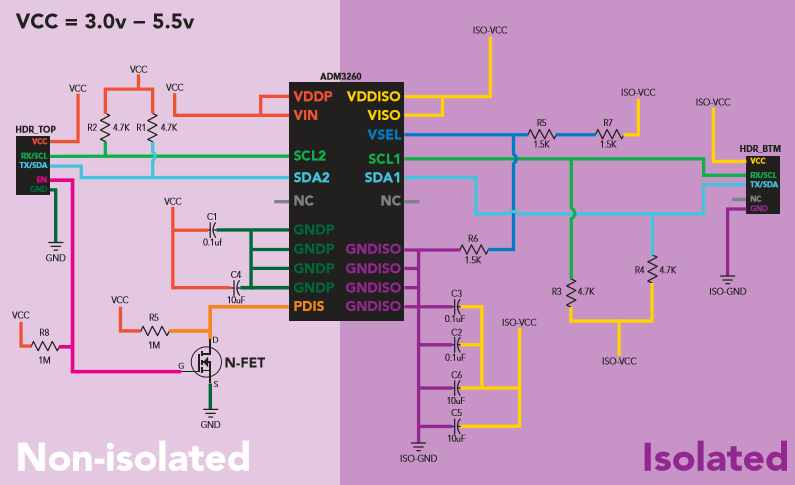
\includegraphics[width=150mm, height=90mm]{Imagenes/2021/imag36.png}
    \caption[Esquema de Funcionamiento del circuito EZO pH]{Esquema de Funcionamiento del circuito EZO pH.\textbf{Fuente: }Pagina Web del Fabricante\cite{ezoph}.}
    \label{fig:4.10}
\end{figure}
En la Figura \ref{fig:4.10} se muestra  el esquema del circuito interno del módulo, cómo están aislados datos y la potencia con el ADM3260, que es el chip encargado de realizar la aislación de los canales I2C utilizados y algunos componentes pasivos. El ADM3260 puede generar una potencia aislada de hasta 150 mW e incorpora dos canales de datos bidireccionales.
Esta tecnología funciona mediante el uso de pequeños transformadores para inducir el voltaje a través de un espacio de aire. Los dos canales de datos tienen una resistencia de extracción de 4.7 k$\Omega$ tanto en las líneas aisladas como en las no aisladas (R1, R2, R3 y R4). El voltaje de salida se configura mediante un divisor de voltaje (R5, R6 y R, 7). produce un voltaje de 3.9V independientemente de su voltaje de entrada.


\textbf{Principio de Operación: }Una sonda de pH mide la actividad del ion de hidrógeno en un líquido, en el extremo inferior de ésta hay una membrana de vidrio que permite a los iones de hidrógeno del líquido que se está midiendo depositarse en la capa exterior del vidrio, mientras que los iones más grandes permanecen en la solución. En la Figura \ref{fig:4.11} se pude apreciar el comportamiento de los iones de hidrógeno de acuerdo al tipo de solución que se tiene. La diferencia en la concentración de iones de hidrógeno (fuera de la sonda y en el interior de la sonda) crea una corriente muy pequeña. Esta corriente es proporcional a la concentración de iones de hidrógeno en el líquido que se mide.
La corriente que se genera a partir de la actividad del ion hidrógeno es el recíproco de esa actividad y se puede predecir usando esta ecuación:
\begin{equation}
E=E^0 + \frac{RT}{F}\times \ln\alpha_{H+} = E^0 - \frac{2.303RT}{F}\rho H
\label{eq:iv}
\end{equation}
Donde $R$ es la constante ideal del gas, $T$ es la temperatura en grados Kelvin y $F$ es la constante de Faraday.
\newline
\hfill
\begin{figure}[t]
\centering
	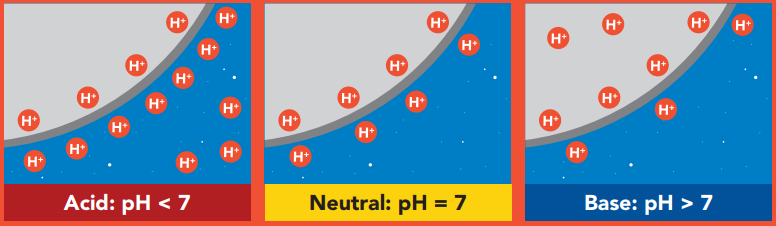
\includegraphics[width=160mm, height=70mm]{Imagenes/2021/imag22.png}%\textwidth%
	\caption[Actividad de los iones de hidrógeno]{Actividad de los iones de hidrógeno.  \textbf{Fuente:}Pagina Web del Fabricante \cite{atlasph}}
	\label{fig:4.11}
\end{figure}

En la Tabla \ref{tab: caract_sondaph} se detallan las características del sensor de pH.
\newline
\hfill
Entre las aplicaciones típicas en las que se utiliza esta sonda están, uso estándar de laboratorio, uso en el campo, en el suelo, cultivos con técnicas de hidroponía o acuaponía, muestras que contienen metales pesados,cerveza, vino y otros.

\begin{table}[H]
\protect\caption[Características del sensor de pH de AtlasScientific]{Características del sensor de pH de AtlasScientific.}
\label{tab: caract_sondaph}
\begin{center}
\begin{tabular}{|l|l|}
\hline
Rango    &  0 - 14\\
\hline
Exactitud      &  +/-0.002\\
\hline
Conector &  BNC macho\\
\hline
Resolución   &  +/-0.0001\\
\hline
Tiempo de Respuesta   &  95\% en 1s\\
\hline
Presión Máxima    &  100PSI\\
\hline
Profundidad Máxima	& 60m\\
\hline
Rango de Temperatura $^{\circ}$C	& 1- 99\\
\hline
Longitud del Cable	& 1m\\
\hline
Sensor de Temperatura Interno	& NO\\
\hline
Tiempo antes de recalibración	& 1 año\\
\hline
Tiempo de Vida	& aprox. 2.5 años\\
\hline
Seguro en Alimentos & Si\\
\hline
Peso & 49 gramos\\
\hline
Dimensiones & 12mm x 150 mm\\
\hline
\end{tabular}
\vspace{5mm}
\newline
\hfill
\textbf{Fuente: }Pagina Web del Fabricante\cite{atlasph}
\end{center}
\end{table} 


\subsection{Sensor de Conductividad}
El sensor utilizado para las lecturas de conductividad se puede apreciar en la Figura \ref{fig:4.12}, también de la empresa Atlas Scientific.
\begin{figure}[t]
\centering
	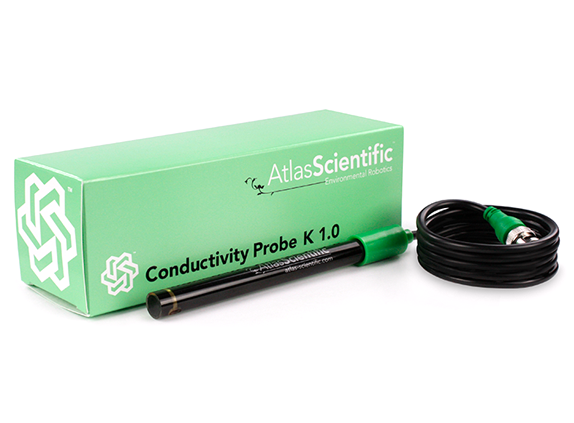
\includegraphics[width=150mm, height=90mm]{Imagenes/2021/imag24.png}%\textwidth%
	\caption[Sensor de CE]{Sensor de CE.  \textbf{Fuente:}Pagina Web del Fabricante \cite{atlasce}}
	\label{fig:4.12}
\end{figure}
Los criterios de selección fueron su extendido uso para control de calidad de aguas para varios usos, buen soporte y extensa documentación disponible en la web, la homogeneidad en los dispositivos electrónicos, al utilizar sensores ya compatibles (Sensor de pH y Sensor de CE) y con los debidos aislamientos requeridos entre estos.  
 
El módulo EZO conductivity Circuit, se muestra en la Figura \ref{fig:4.13} emplea un método de resolución de escala. A medida que aumenta la conductividad, la resolución entre lecturas disminuye como se puede apreciar en la Tabla \ref{tab:resol_ce}.
\begin{figure}[b]
    \centering
    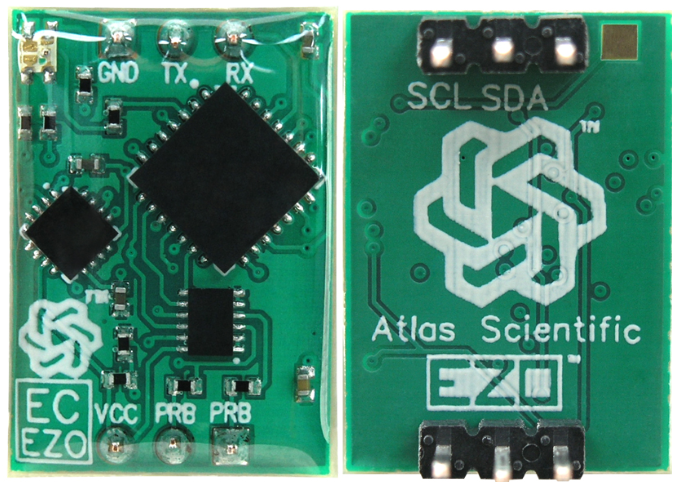
\includegraphics[width=70mm, height=60mm]{Imagenes/2021/imag28.png}
    \caption[EZO conductivity Circuit]{EZO conductivity Circuit. \textbf{Fuente: }Página Web del Fabricante.}
    \label{fig:4.13}
\end{figure}
El módulo emitirá lecturas de conductividad donde los primeros 4 dígitos son válidos y los demás se establecen en 0. Esto excluye las lecturas de conductividad que son menores a 9.99. En ese caso, solo se emitirán 3 dígitos de conductividad.

\begin{table}[t]
    \protect\caption[Resolución de Escala Sensor de Conductividad]{Resolución de Escala Sensor de Conductividad.}
    \label{tab:resol_ce}
    \centering
    \begin{tabular}{|c|c|}
           \hline
         \textbf{Valor}&\textbf{Resolución}  \\
         \hline
         0.07-99.99 & 0.01$ \mu S/cm$ \\
         \hline
         100.1-999.9 & 0.1 $\mu S/cm $\\
         \hline
         1,000-9,999 & 1.0 $\mu S/cm$ \\
         \hline
         10,000-99,990 & 10.0 $\mu S/cm $\\
         \hline
         100,000-999,99 & 100 $\mu S/cm$ \\
         \hline
    \end{tabular}
   \vspace{5mm}
   \newline
   \hfill \textbf{Fuente: }\cite{ezoce}.
\end{table}

\textbf{Principio de operación: }
Una sonda de conductividad eléctrica (CE) mide la conductividad eléctrica en una solución. Se usa comúnmente en ecosistemas de agua dulce para controlar la cantidad de nutrientes, sales o impurezas en el agua.
Dentro de la sonda de conductividad, dos electrodos se colocan opuestos entre sí como se muestra en la Figura \ref{fig:4.14}, se aplica un voltaje de CA a los electrodos, lo que hace que los cationes se muevan al electrodo cargado negativamente, mientras que los aniones se mueven al electrodo positivo. Cuanto más electrolito libre contiene el líquido, mayor es la conductividad eléctrica.

\begin{figure}[H]
    \centering
    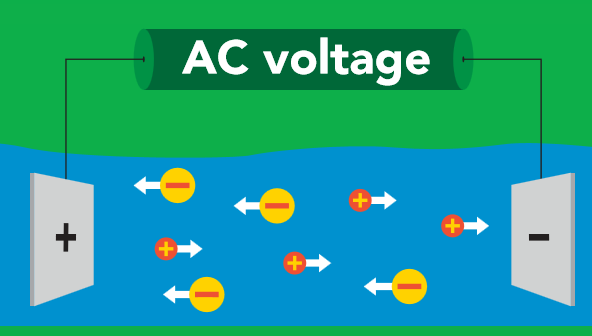
\includegraphics[width=90mm, height=60mm]{Imagenes/2021/imag37.png}
    \caption[Principio de Funcionamiento del Sensor de Conductividad]{Principio de Funcionamiento del Sensor de Conductividad. \textbf{Fuente: }\cite{ezoce}.}
    \label{fig:4.14}
\end{figure}

En la Tabla \ref{tab:caract_ce} se muestran las principales características del sensor de conductividad.
Entre los usos comunes de este sensor se encuentran el uso estándar en laboratorio, uso en el campo, en acuaponía, hidroponía y en acuarios.
\begin{table}[H]
\protect\caption[Características del sensor de CE de AtlasScientific]{Características del sensor de CE de AtlasScientific.}
\label{tab:caract_ce}
\begin{center}
\begin{tabular}{|l|l|}
\hline
Rango    &  5 - 200.000 $\mu S\/cm$\\
\hline
Exactitud      &  +/-2\% \\
\hline
Conector &  BNC macho\\
\hline
Resolución   &  +/-0.0001\\
\hline
Tiempo de Respuesta   &  90\% en 1s\\
\hline
Presión Máxima    &  3,447 kPa (500 PSI) \\
\hline
Profundidad Máxima	& 343 metros\\
\hline
Rango de Temperatura $^{\circ}$C	& 1- 110\\
\hline
Longitud del Cable	& 1m\\
\hline
Sensor de Temperatura Interno	& NO\\
\hline
Tiempo antes de recalibración	& 10 año\\
\hline
Tiempo de Vida	& aprox. 10 años\\
\hline
Dimensiones	& 12mm x 152mm\\
\hline
Peso	& 51 gramos\\
\hline
Superficie de medición	& Grafito\\
\hline
Seguro en Alimentos	& Si\\
\hline
\end{tabular}
\vspace{5mm}
\newline
\hfill \textbf{Fuente:} \cite{atlasce}
\end{center}
\end{table}

%%%%%%%%%%%%%%%%%%%%%%%%CAMBIAR
\subsection{Sensor de Temperatura}
En la Figura \ref{fig:4.15}  se puede apreciar el sensor de Temperatura utilizado fabricado por la empresa Atlas Scientific.


\begin{figure}[t]
    \centering
    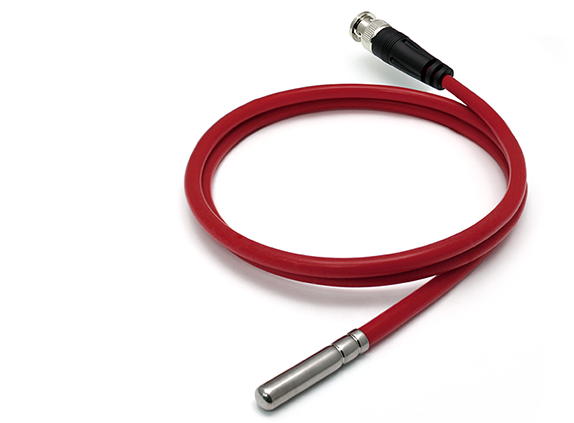
\includegraphics[width=90mm, height=70mm]{imagenes/imag39.png}
    \caption[Sensor de Temperatura PT 1000]{Sensor de Temperatura PT 1000. \textbf{Fuente: } Página Web del Fabricante. }
    \label{fig:4.15}
\end{figure}


\textbf{Principio de Operación: }
A diferencia de cualquier otro material, la correlación entre la resistencia y la temperatura en el platino es bastante lineal. Es por esta razón que el sensor de temperatura RTD de platino es el estándar industrial para la medición de temperatura.

La sonda de temperatura PT-1000 es un termómetro tipo resistencia. Donde PT significa platino y 1000 es la resistencia medida de la sonda a 0$^{\circ}$C en $\Omega$ (1k a 0$^{\circ}$C).
A medida que la temperatura cambia, la resistencia del platino cambia.
Para convertir la resistencia de la sonda a la temperatura, se utiliza la siguiente ecuación simplificada

\begin{equation}
    T=-\frac{\sqrt{(-0.00232(R)+17.59246)}-3.908}{0.00116}
\end{equation}

Donde $T$ esta en grados Celsius y $R$ es el valor de la resistencia medida por el sensor.

El módulo utilizado para el tratamiento de las señales es el mostrado en la Figura \ref{fig:4.16} también fabricado por la empresa Atlas Scientific.
\begin{figure}[t]
    \centering
    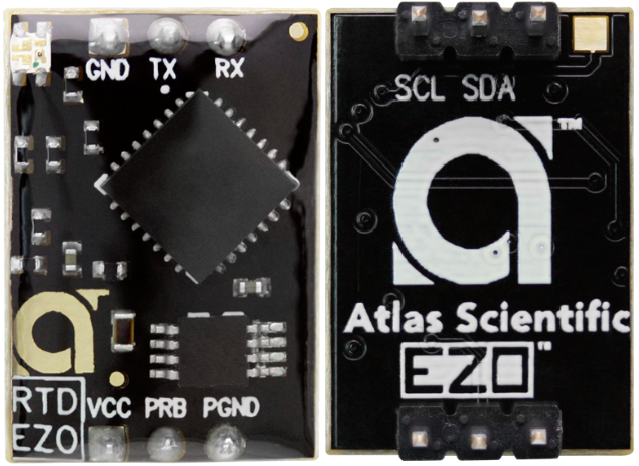
\includegraphics[width=90mm, height=70mm]{imagenes/imag38.png}
    \caption[EZO-RTD Circuito Integrado de Temperatura]{EZO-RTD Circuito Integrado de Temperatura.\textbf{Fuente: }Pagina Web del Fabricante.}
    \label{fig:4.16}
\end{figure}
Es un sistema informático de tamaño reducido que está diseñado específicamente para ser utilizado en aplicaciones donde se requiera mediciones exactas y precisas de la temperatura a través de una sonda de temperatura genérica PT-100 / PT-1000. Se conecta directamente a la placa Tentacle T3 y no necesita de aislamiento a diferencia de los otros módulos de sensores.

En la Tabla \ref{tab:caract_temp} se visualizan las características del Sensor de Temperatura PT-1000.
Entre las aplicaciones de uso común de este sensor están el uso estándar de laboratorio, uso en el campo, en el suelo, acuaponía, hidroponía, en bebidas como cerveza, vino u otro licor.
%%%%%%%%%%%%%%%%%%%%%%%%%%%%%%%%%%%%

\section[Bloque de Alimentación]{Bloque de Alimentación}

Para lograr autonom\'ia energ\'etica para la sonda se opto por utilizar bater\'ias LiPo Nano-Tech por sus caracter\'isticas t\'ecnicas que permitir\'an alimentar de forma suficiente a toda los componentes que conforman la sonda, como se aprecia en la Figura \ref{fig:4.17}. 

Las baterias Turnigy nano-tech Lipoly bater\'ias fueron dise\~nados para alto rendimiento . Utilizando un avanzado sustrato electrones que permite pasar m\'as libremente de \'anodo a c\'atodo con menos impedancia interna.
 Las ventajas que presenta la utilización de esta fuente son la posibilidad de tener tensiones de +/- 3.3V, +/-5V y +/-12V sin la necesidad de realizar circuitos para la obtención de estos voltajes en comparación a la utilización de baterías de litio.
 \newline
 \hfill
Las ventajas sobre las bater\'ias tradicionales LIPOLY;
\begin{itemize}
    \item La densidad de potencia alcanza 7,5 kW / kg.
    \item Menos hueco de tensi\'on durante la descarga de alta velocidad, dando m\'as poder bajo carga.
    \item Impedancia interna puede llegar tan bajo como 1.2 m${\Omega }$ en comparación con la de 3 m${\Omega }$ de un Lipoly estándar
    \item Control t\'ermico m\'as, paquete por lo general no supera 60 $^{\circ}$C.
    \item Hinchazón durante la carga pesada no supera 5\%, en comparación con 15\% de un Lipoly normal.
    \item Mayor capacidad durante la descarga pesada. M\'as del 90\% a la tasa de 10O\% C.
    \item Carga r\'apida capaz, hasta 15$^{\circ}$C en algunas baterías.
    \item Mayor duraci\'on del ciclo, casi el doble que el de la tecnolog\'ia LiPoly est\'andar.
\end{itemize}


La tecnolog\'ia de nano-core en las bater\'ias de litio es la aplicaci\'on de aditivos conductores nan\'ometros. Los aditivos nan\'ometros conductora forman redes ultra-fuertes de electrones de conducci\'on en los electrodos que pueden aumentar la conductividad electr\'onica.

Estos aditivos crean la capacidad de imbibici\'on en el l\'iquido portador para suministrar m\'as canales de iones. Esto mejora la capacidad de transmisi\'on de iones y la difusi\'on de iones. A trav\'es de la mejora de la conductividad y de iones de transmisi\'on electr\'onica, la impedancia se reduce y la polarizaci\'on de la descarga de alta tasa disminuye en gran medida.

 \newline
 \hfill
\begin{table}[t]
\protect\caption[Caracter\'isticas de bateria Lipo Nano-Tech ]{Caracter\'isticas de bateria Lipo Nano-Tec 5100mAh.}
\label{tab:caract_bat}
\begin{center}
\begin{tabular}{|l|l|}
\hline
Capacidad    &  5100 mAh \\
\hline
Voltaje      &  2S3P/ 7.4 V \\
\hline
Descarga &  65C / 135C \\
\hline
Peso  & 290 g\\
\hline
Dimensi\'on   &  69x47x25 mm\\
\hline
Conector equilibrio	& JST\\
\hline
\end{tabular}
\vspace{5mm}
\newline
\hfill \textbf{Fuente:} Pagina Web del Fabricante\cite{bateria}
\end{center}
\end{table}




\begin{figure}[H]
\centering
	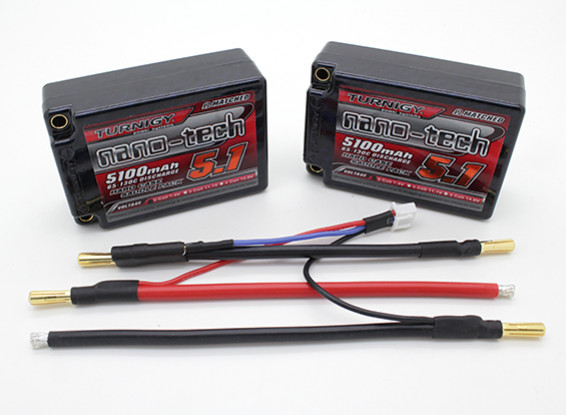
\includegraphics[width=90mm, height=70mm]{Imagenes/2021/imag29.jpg}%\textwidth%
    \caption[Bateria Turnigy Nano]{Bateria Turnigy Nano.\textbf{Fuente: } Pagina Web del Fabricante\cite{bateria}.}
	\label{fig:4.17}
\end{figure}



 En contrapartida, limitará a nuestro sistema, ya que deberá ir conectado a la red eléctrica todo el tiempo que se requiera del uso de la misma.



\section[Características Técnicas de los módulos]{Características Técnicas del módulo Sonda}
La Tabla \ref{tab:carac_general} detalla las características técnicas del mecanismo a ser desarrollado, teniendo en cuenta los objetivos planteados en la Sección 1.3.

\begin{table}[H]
\protect\caption[Datos Técnicos]{Datos Técnicos. \label{tab:carac_general}}
    \centering
    \scalebox{0.9}{\begin{tabular}{|c|c|}
        \hline
        \textbf{Característica} & \textbf{Valor}  \\
        \hline
        \multicolumn{2}{|c|}{\textbf{Sensores}} \\
        \hline
        Cantidad & $ 5 $   \\
        \hline
        \multicolumn{2}{|c|}{\textbf{Físico}} \\
        \hline
        Dimensiones & $< 50 [cm]$  $< \phi 15[cm]$   \\
        \hline
        Peso &  $ > 6 kg$ \\
        \hline
        Caja Electrónica & Herm\'etica  \\
        \hline
        \multicolumn{2}{|c|}{\textbf{Eléctrico}} \\
        \hline
         Alimentación & 5 V DC  \\
        \hline
         Autonomía & LiPo 5100mAh  \\
        \hline
         \multicolumn{2}{|c|}{\textbf{Interfaz}} \\
         \hline
         Configuración de Parámetros & Por Interfaz Gráfica, SSH, VNC  \\
        \hline
         Transmisi\'on Remota  & Si  \\
        \hline
    \end{tabular}}
    \vspace{5mm}
    \newline
    \hfill \textbf{Fuente:} Elaboración Propia
\end{table}

\begin{table}[t]
\protect\caption[Funciones Generales]{Funciones Generales. \label{tab:fun_general}}
    \centering
    \begin{tabular}{|l|l|l|}
        \hline
        \textbf{Descripción} & \textbf{Decisión} & \textbf{Característica} \\
        \hline
         Comunicaci\'on  Perif\'ericos  & Algoritmo comunicaci\'on & \multicolumn{1}{|l|}{\begin{tabular}[c]{@{}l@{}} Env\'io y recipci\'oon de estados \\ funcionamiento y datos de los \\ dispositivos conectados a la red \end{tabular}}
         \\
        \hline
        Lectura de Sensores & Algoritmo muestreo & \multicolumn{1}{|l|}{\begin{tabular}[c]{@{}l@{}} Se Lectura secuencial de los\\ sensores pH, CE,\\ OD, OPR, T\end{tabular}}
         \\
        \hline
        Almacenamiento datos & Algoritmo datos &
        \multicolumn{1}{|l|}{\begin{tabular}[c]{@{}l@{}} Consulta y registro as\'incrono \\ 
        del muestreo\end{tabular}}
          \\
        \hline
        Transmisi\'on datos  & Algoritmo transmisi\'on &
        \multicolumn{1}{|l|}{\begin{tabular}[c]{@{}l@{}} Transmisi\'on asincr\'onica \\ a estaci\'on remota \end{tabular}}
           \\
        \hline
    \end{tabular}
    \vspace{5mm}
    \newline
    \hfill \textbf{Fuente:} Elaboración Propia
\end{table}

\section{Descripci\'on  sistema }

\section[Descripción General del Sistema]{Descripción General del Sistema}

En referencia al modelo conceptual del sistema, éste está constituido, en general, por una Interfaz de Usuario, un bloque de Control, un bloque de Sensores, un bloque de actuadores y un bloque de Alimentación  como se pude apreciar en la Figura \ref{fig:4.1}.



\section[Características Técnicas de los módulos]{Características Técnicas del módulo Despliegue}
La Tabla \ref{tab:carac_general} detalla las características técnicas del mecanismo a ser desarrollado, teniendo en cuenta los objetivos planteados en la Sección 1.3.
\begin{table}[H]
\protect\caption[Datos Técnicos]{Datos Técnicos. \label{tab:carac_general}}
    \centering
    \scalebox{0.9}{\begin{tabular}{|c|c|}
        \hline
        \textbf{Característica} & \textbf{Valor}  \\
        \hline
        \multicolumn{2}{|c|}{\textbf{F\'isico}} \\
        \hline
        Capacidad de carga & $ > 10 [Kg] $   \\
        \hline
        Dimensiones & $< 50 [cm]$  x $50 [cm]$ x $50 [cm]$    \\
        \hline
        Peso &  $ < 15 kg$ \\
        \hline
        Caja Electrónica & Herm\'etica  \\
        \hline
        \multicolumn{2}{|c|}{\textbf{Eléctrico}} \\
        \hline
         Alimentación & 12 V DC  \\
        \hline
         Autonomía & No  \\
        \hline
         \multicolumn{2}{|c|}{\textbf{Interfaz}} \\
         \hline
         Configuración de Parámetros & Por Interfaz Gráfica  \\
        \hline
         Transmisi\'on Remota  & Si  \\
        \hline
    \end{tabular}}
    \vspace{5mm}
    \newline
    \hfill \textbf{Fuente:} Elaboración Propia
\end{table}


\section{Aspectos Generales}
El desarrollo de la sonda implic\'o una serie de desaf\'ios t\'ecnicos, por ese motivo esa secci\'on se organiza de la siguiente manera

\begin{itemize}
    \item Dise\~no Mec\'anico: abarca todos los criterios considerados al dise\~no de la sonda y sistema de despliegue. 
    \item Fabricaci\'on Mec\'anica: abarca las t\'ecnicas y materiales empleadas para la fabricaci\'on de los componentes.
    \item Programaci\'on e Integraci\'on de los sensores: en esta secci\'on abarca lo referente a los distintos script desarrollados para lograr el funcionamiento del dispositivo.
\end{itemize}

\section{Dise\~no Mec\'anico}
Para el proceso de dise\~no se siguieron los procedimientos de XXX donde agrupan el proceso de dise\~no en las siguientes etapas:
Etapas del dise\~no: 

\subsection{Sonda}
\subsubsection{Conceptualizaci\'on}
Conceptualmente se definen los requerimientos m\'inimos para el correcto funcionamiento de la sonda.
\begin{itemize}
    \item versatilidad: su implementación debe de ser independiente a la dispositivo de soporte, pudiendo operar en cualquier medio de transporte.
    \item 
    \item Energ\'ia: la donde deber\'a tener autonom\'ia energ\'etica para sus operaciones de monitoreo,  
\end{itemize}
la donde deberá de contener en su interior al menos cinco sensores  (ph,CE,OD,OPR,T), adem\'as de toda la electr\'onica necesaria para la operaci\'on de estos. La sonda deber\'a tener autonom\'ia energ\'etica y poder sumergirse hasta una profundidad m\'inima de 5 metros , teniendo en cuenta que la profundidad promedio del lago Ypakarai es de 3 metros [\cite{hidrologiaItaipu}].
   
\subsubsection{An\'alisis}
En base a las conceptualizaci\'on de la secci\'on aterior y los materiales disponibles en el pa\'is se concluyen  :




\subsection{Despliegue}
\subsubsection{Conceptualizaci\'on}

deber\'a brindar soporte para que la sonda pueda hacer mediciones a varios niveles, dise\~no simple y adaptativo para ser instalado en embarcaciones de investigaci\'on.

\subsubsection{An\'alisis}
En base a las conceptualizaci\'on de la secci\'on aterior y los materiales dispobibles en el pa\'is se concluyen  :
\begin{itemize}
    \item Sonda: .
    \item Despliegue: deber\'a brindar soporte para que la sonda pueda hacer mediciones a varios niveles, dise\~no simple y adaptativo para ser instalado en embarcaciones de investigaci\'on.
\end{itemize}


\section{Fabricaci\'on de la Sonda.}

\subsection{Diseño, Mecanizado de Piezas}
El diseño final de la sonda, fue el resultado de varias versiones que fueron modificándose de tal manera que resulte mejor y se adapte a los requerimientos del proyecto.
Partiendo de un diseño de un misil militar por su dise\~no din\'amico , similar al propuesto por [1], modificado hasta la versión final con el cual se realizaron las pruebas. Su diseño modular esta pensado para el caso que se le requiera sacar o añadir uno o mas sensores, se pueda seguir utilizando la sonda con cambios mínimos para adaptación.
La primera sonda fue impresa en su totalidad con una impresora 3D, en material Acrilonitrilo butadieno Estireno(ABS), por sus propiedades de alta resistencia al impacto y su baja degradación en presencia de líquidos. 
El diseño de la sonda (Sonda V4.3) utilizado en el Cormoran-I, esta disen\~ado para ser albergar a seis sensores específicos de la empresa Atlas Scientific.

\begin{itemize}
    \item Sonda PH de Plata/cloruro de plata de calidad científica, EZO pH Circuit.
    \item Sonda ORP de barra de platino, EZO OPR Circuit.
    \item Sonda de conductividad: 5 [\(\mu S/cm\)] a 200,000 [\(\mu S/cm\)], EZO Conductivity Circuit.
    \item EZO RGB, Sensor de color integrado 8bit.
    \item Sonda de oxígeno disuelto, EZO OD Circuit.
    \item Sensor de Temperatura DS18B20. Sparkfun.
\end{itemize}
    
\subsection{Versiones de la Sonda }
Se desarrollaron cuatro versiones de la sonda, con el programa de diseño CAD 3D SolidWorks 2015. La sonda es un un ensamble de tres piezas principales, denominadas:

\begin{itemize}
\item \textbf{Frente} : Pieza frontal de la sonda, la función de esta pieza es principalmente de protección contra basura o objetos que puedan dañar a los sensores. Se diseño de forma cilíndrica hueca de base circular para las versiones de la sonda Figura1-a y Figura1-b, las de base elipsoidal para las versiones Figura1-d y Figura1-e, Posee ranuras laterales para que el agua ingrese dentro de la cavidad hueca de esta pieza y los sensores puedan hacer las mediciones.  
\item \textbf{Anillo} : Pieza central de la sonda y enlace de las otras dos piezas, la función de esta pieza es servir de soporte a las sensores y posicionarlos de forma horizontal. En el caso que se requiera otros sensores, esta es la única pieza que tendría que ser adaptado a los nuevos sensores.
\item \textbf{Base}  : Pieza posterior de la sonda, su función es de protección de los cables de los sensores. 
\end{itemize}

\begin{enumerate}
\item \textbf{Sonda V0.0:} La versión inicial de la sonda, con diseño cilíndrico de base circular, el inconveniente principal de este diseño fue la debilidad estructural de la parte frontal de la sonda por la cantidad de ranuras, ademas el diseño de la punta dificultaba bastante para ser impreso en la impresora 3D.
\item \textbf{Sonda V1.0:} La siguiente versión, resolvía los problemas de debilidad estructural de la parte frontal espaciando mas las ranuras y reemplazando la punta de la pieza frontal con un diseño mas redondeado para que pueda ser impresa con mayor facilidad.   
\item \textbf{Sonda V2.0:} En esta versión de la sonda, se probaron con otras geometrías para mejorar la dinámica del fluido, de esta forma cargar menos al motor propulsor del Dron. El inconveniente de este diseño fue, que por su geometría era mas grande que el anterior por tanto utilizaba mas material.
\item \textbf{Sonda V3.0:} La siguiente versión se opto por una base elipsoidal para la sonda, ademas se agrego al diseño un soporte para que pueda ser fijado al Dron con tornillos en la parte inferior, se realizaron cambios en la base para crear un ensamble mas dinámico. Fue la primera aproximación para el diseño final, el inconveniente de esta sonda era el soporte que resultaba poco practico de implementar y podría causar daños estructurales al casco del dron.
\item \textbf{Sonda V4.0:} La ultima versión resuelve el problemas de soporte, al agregar un riel en la parte superior de toda la sonda para fijarlo cuando se requiera al dron sin la utilización de tornillos o algún elemento fijador que pueda dañar el casco del dron.
\item \textbf{Sonda V4.1:} En la primera modificación de la versión 4 de la sonda, se optimizo el tamaño de la pieza frontal de la sonda,  para utilizar menos material y ofrecer mayor protección a las puntas de los sensores.
\item \textbf{Sonda V4.2:} En la segunda revisión de la versión 4, se re diseño la parte posterior de la sonda, para reemplazar el sistema modo inicial que conectar los sensores al dron, que en las versiones anteriores se encontraba en la parte superior, y como esta versión se diseña el riel, se opto por hacer por una perforación e la base para que por ella pueda conectarse al Dron.
\item \textbf{Sonda V4.3:} En la ultima revisión de la versión 4, se re diseña la pieza central de la sonda para agregarle un juego de juntas de gomas circulares, por los agujeros preparados para los sensores para de esta forma ejercer sobre ellos un mejor agarre, ademas se modifica la dimensión de sensor ubicado en la parte central de la pieza.
\end{enumerate}


\begin{figure}[htbp]
\centering
\subfigure[V0.0]{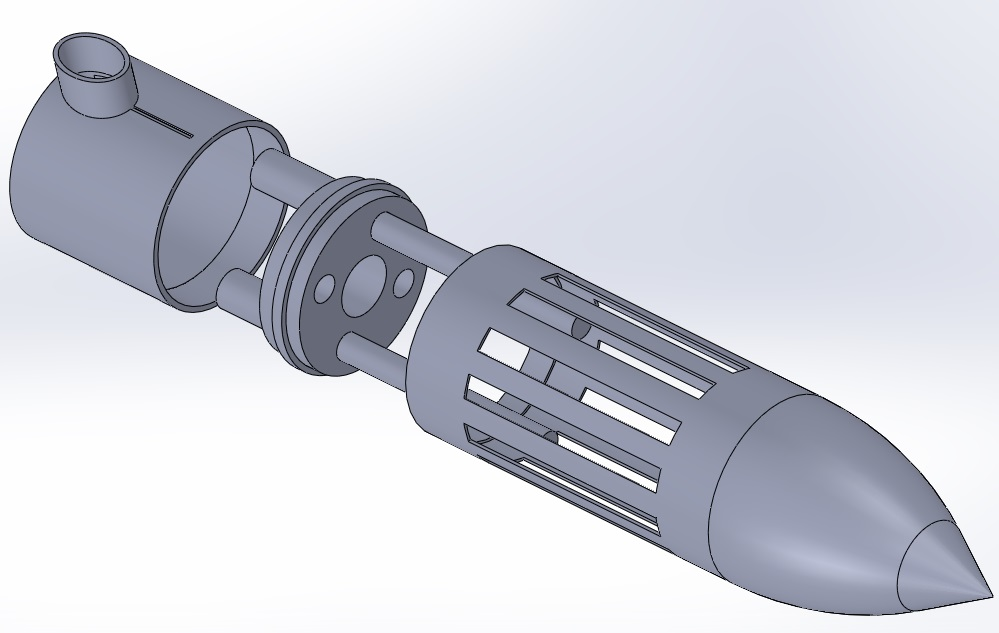
\includegraphics[width=50mm]{Imagenes/Sonda_v0.jpg}}

\subfigure[V1.0]{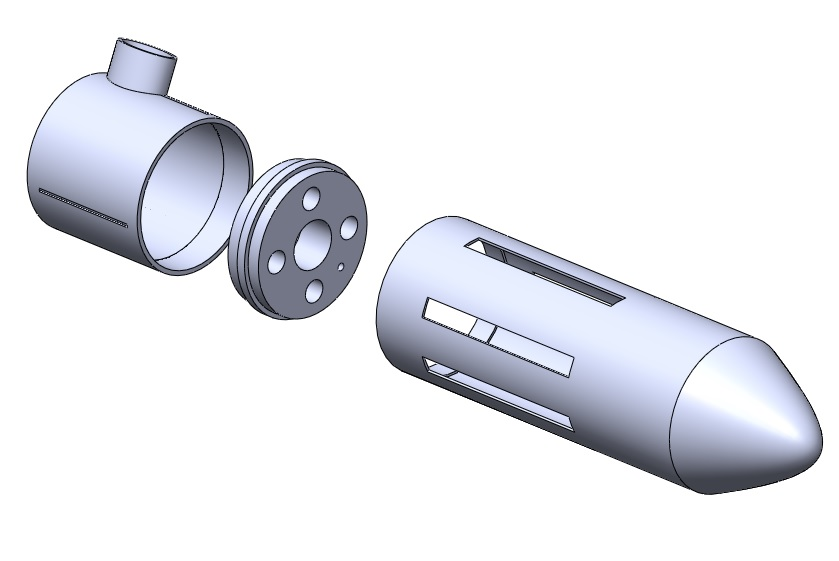
\includegraphics[width=50mm]{Imagenes/Sonda_v1.jpg}}

\subfigure[V2.0]{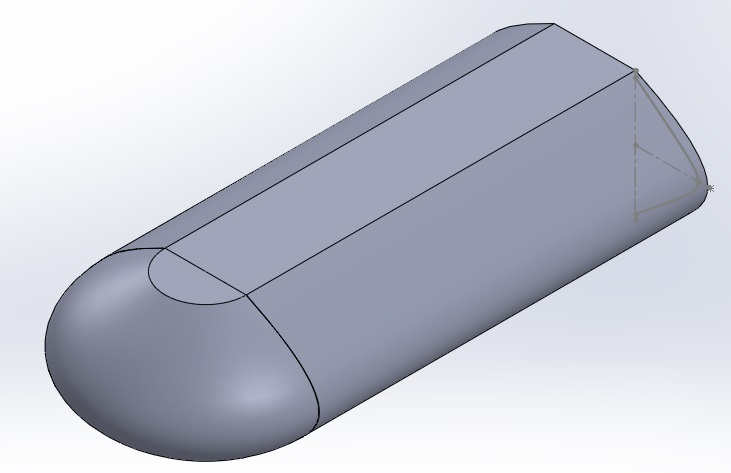
\includegraphics[width=50mm]{Imagenes/Sonda_v2.jpg}}

\subfigure[V3.0]{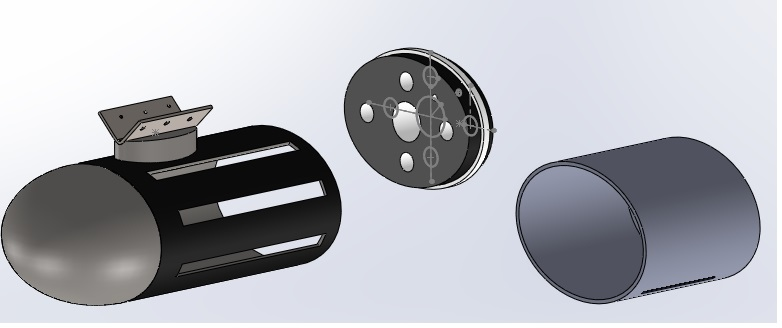
\includegraphics[width=50mm]{Imagenes/Sonda_v3.jpg}}

\subfigure[V4.0]{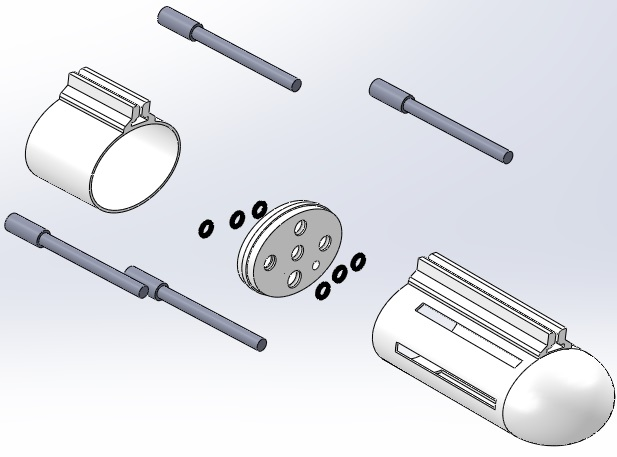
\includegraphics[width=50mm]{Imagenes/Sonda_v4.jpg}}

\caption{Versiones Sonda. Fuente: elaboración propia} \label{fig:Sonda_Versiones}
\end{figure}

\begin{figure}[htbp]
\centering
\subfigure[V4.3 . Frontal]{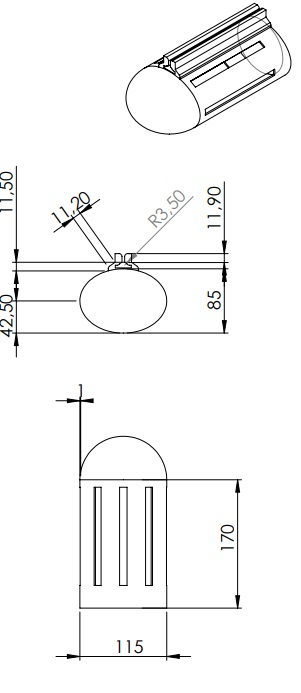
\includegraphics[width=40mm]{Imagenes/Sonda_v4_1.jpg}}

\subfigure[V4.3 . Anillo]{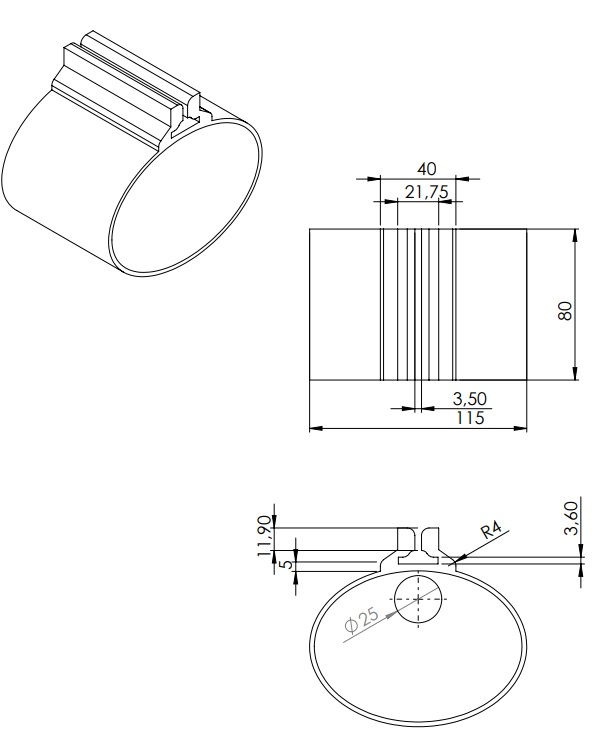
\includegraphics[width=40mm]{Imagenes/Sonda_v4_2.jpg}}

\subfigure[V4.3 . Base]{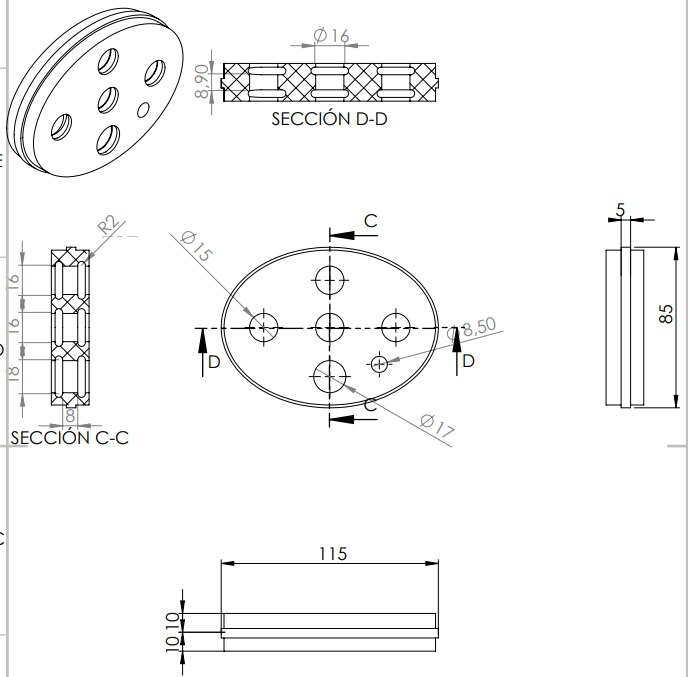
\includegraphics[width=40mm]{Imagenes/Sonda_v4_3.jpg}}

\caption{Versiones Sonda. Fuente: elaboración propia} \label{fig:Sonda_Versiones}
\end{figure}

\section{Sonda v5.0}
Para el proyecto PINV15-177, se deberán realizar una serie de cambios al modelo final de la sonda utilizado en el CORMORAN-I, por la operación a multivinel, el material a ser utilizado y la ubicación de la electrónica.
\subsection{Operación Multinivel}
Como se introduce la capacidad de poder censar a multiniveles, es necesario cambiar el tipo de material de construcción para que de esta forma se pueda sumergir con su propio peso, y no requiera de otro medio externo para sumergirse. 
\subsection{Sonda Embebida}
Considerando que la versión 4.3, la sonda se fija por el casco del dron, el circuito de control y la base de datos se ubica dentro del dron, y los sensores de la sonda se conectan mediante cables coaxiales, segun datos proveídos por el informe de batimetria, realizado en el agosto del 2014  por la Dirección de Coordinación Ejecutiva del Centro Internacional de Hidroinformatica (CIH) dependiente de la Hidroeléctrica Itaipu, la máxima profundidad del lago Ypakarai es de 3,226[m], para la operación multinivel para estas profundidades la implementacion de versión actual resulta poco practica ya que se requerirán cables mas largos, expuestos al ambiente, agua, tracción pudiendo dañarse o registrar lecturas erróneas.\\ Para subsanar este inconveniente se propone que todo la electrónica se encuentre dentro de la sonda, en la parte posterior o base, de esta forma ademas eliminar el uso de cables, la sonda por si sola ya sera capaz de operar.

\subsection{Primera Versi\'on sonda Embebida}

\subsection{Diseño - Modelado}
El dise\~no y modelado de la sonda se realizo, utilizando el software de modelacion 3D SolidWorks.
El realizo el diseño de forma modular, de tal forma que que la sonda se adaptar con cambios mínimos en el caso de ser requerido, ante posibles cambios de configuración como ser, adición de otro sensor o modo de operación.    
La sonda consta de tres partes o módulos principales:

\begin{itemize}
\item \textbf{Base}: Modulo no reemplazable, a fabricarse en acero inoxidable, en esa sección de la sonda se almacenara toda la electrónica de control, procesamiento de señales provenientes de los sensores, alimentación y la base de datos de las lecturas registradas por los sensores. Este modulo debe de ser hermético 

\item \textbf{Anillo}: Modulo reemplazable, a ser fabricado de acero inoxidable, parte central de la sonda, la función de esta pieza es de mantener a los sensores posicionados correctamente y cumple la función de sello para la base, de esta forma cerrar de forma hermética la base.

\item \textbf{Envolvente}: Modulo reemplazable, a ser fabricado en material ácido poliláctico  láctico (PLA), la envolvente es un pieza que rodea todo la otros dos módulos, y su función principal es de proteger la parte frontal de los sensores y mejorar la dinámica del fluido mediante su geometría impreso totalmente en impresora 3D.  

\end{itemize}

\begin{figure}[h]
\fbox{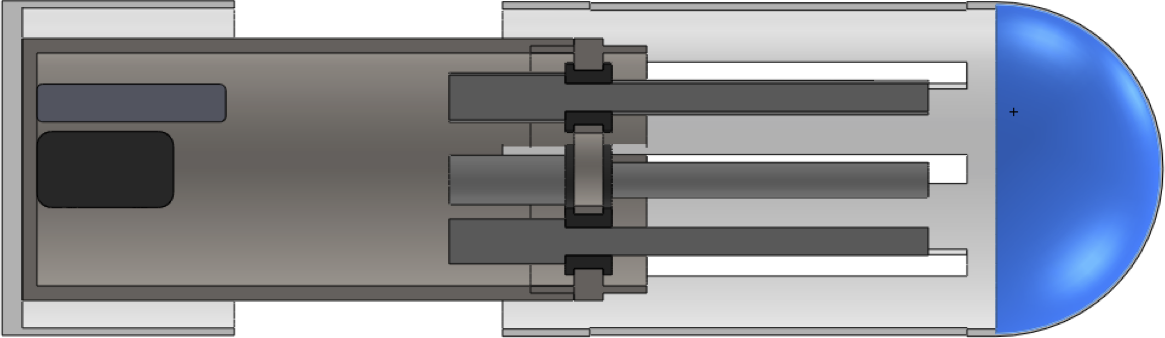
\includegraphics[scale=0.4]{Imagenes/2019/CompletoV5_0555.png} }
\caption{Dise\~no Sonda Completa. Fuente: elaboración propia}
\label{fig:SondaV5}
\end{figure}

\begin{figure}[h]
\fbox{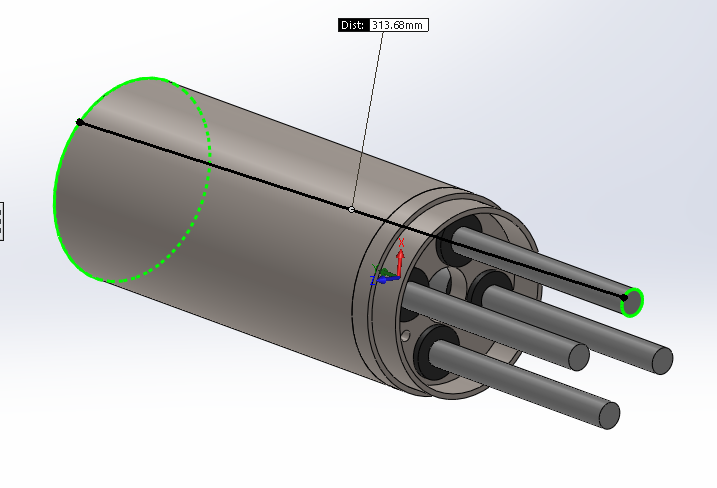
\includegraphics[scale=0.4]{Imagenes/2019/misilv5a.png} }
\caption{Dise\~no Base y anillo. Fuente: elaboración propia}
\label{fig:SondaV5}
\end{figure}

\section{Sonda V6.0}
\subsection{Diseño - Modificaciones}
Por la falta de materiales del diseño anterior se realizar\'on modif\'idicaciones para poder fabricar con materiales que s\'i pudimos conseguir en el pa\'is, en el diseño anterior estaba pensado fabricar la sonda en acero inoxidable.
El material utilizado fue Nylon que requiri\'o de un rediseño de la sonda conformada por dos elementos principales denominados base y anillo. \\ 

\textbf{Base: }
Para una mejor robustez la base, se ensancharon las paredes internas y se diseño  con  rosca interna Whitworth fina.\\ 
\begin{figure}[h]
\centering
\fbox{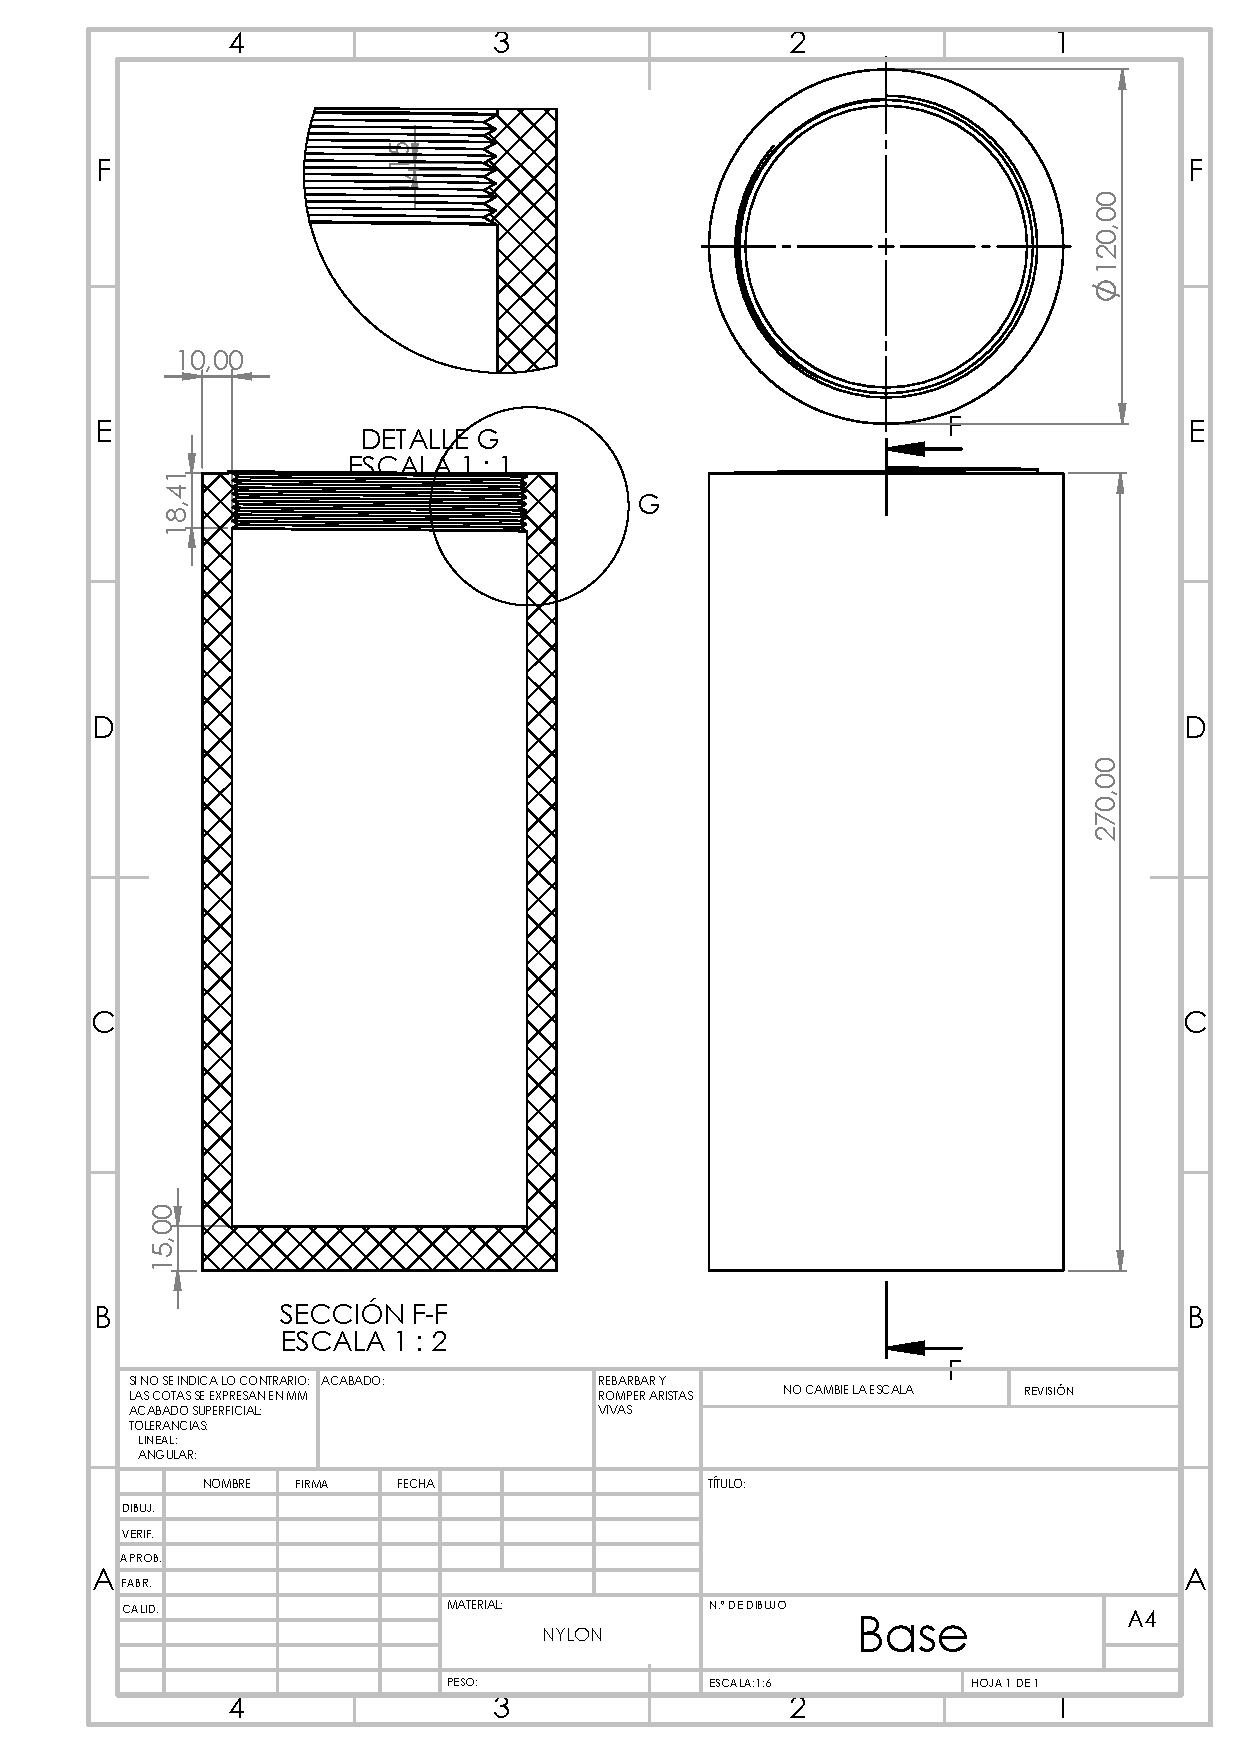
\includegraphics[scale=0.35]{Imagenes/2019/Base2019.PDF} }
\caption{Dise\~no final de la base. Fuente: elaboración propia}
\label{fig:Base2019}
\end{figure}

\textbf{Anillo: }
El diseño anterior Figura: \ref{fig:SondaV5}, se contemplaba el uso de O-ring para el sellado de la sonda, por las dificultades t\'ecnicas para la fabricaci\'on de las ranuras necesarias se opto por otro dispositivo de sellado denominado,  reten hidr\'aulico, dos reten hidr\'aulico por abertura de cada sensor
\\
\begin{figure}[h]
\centering
\fbox{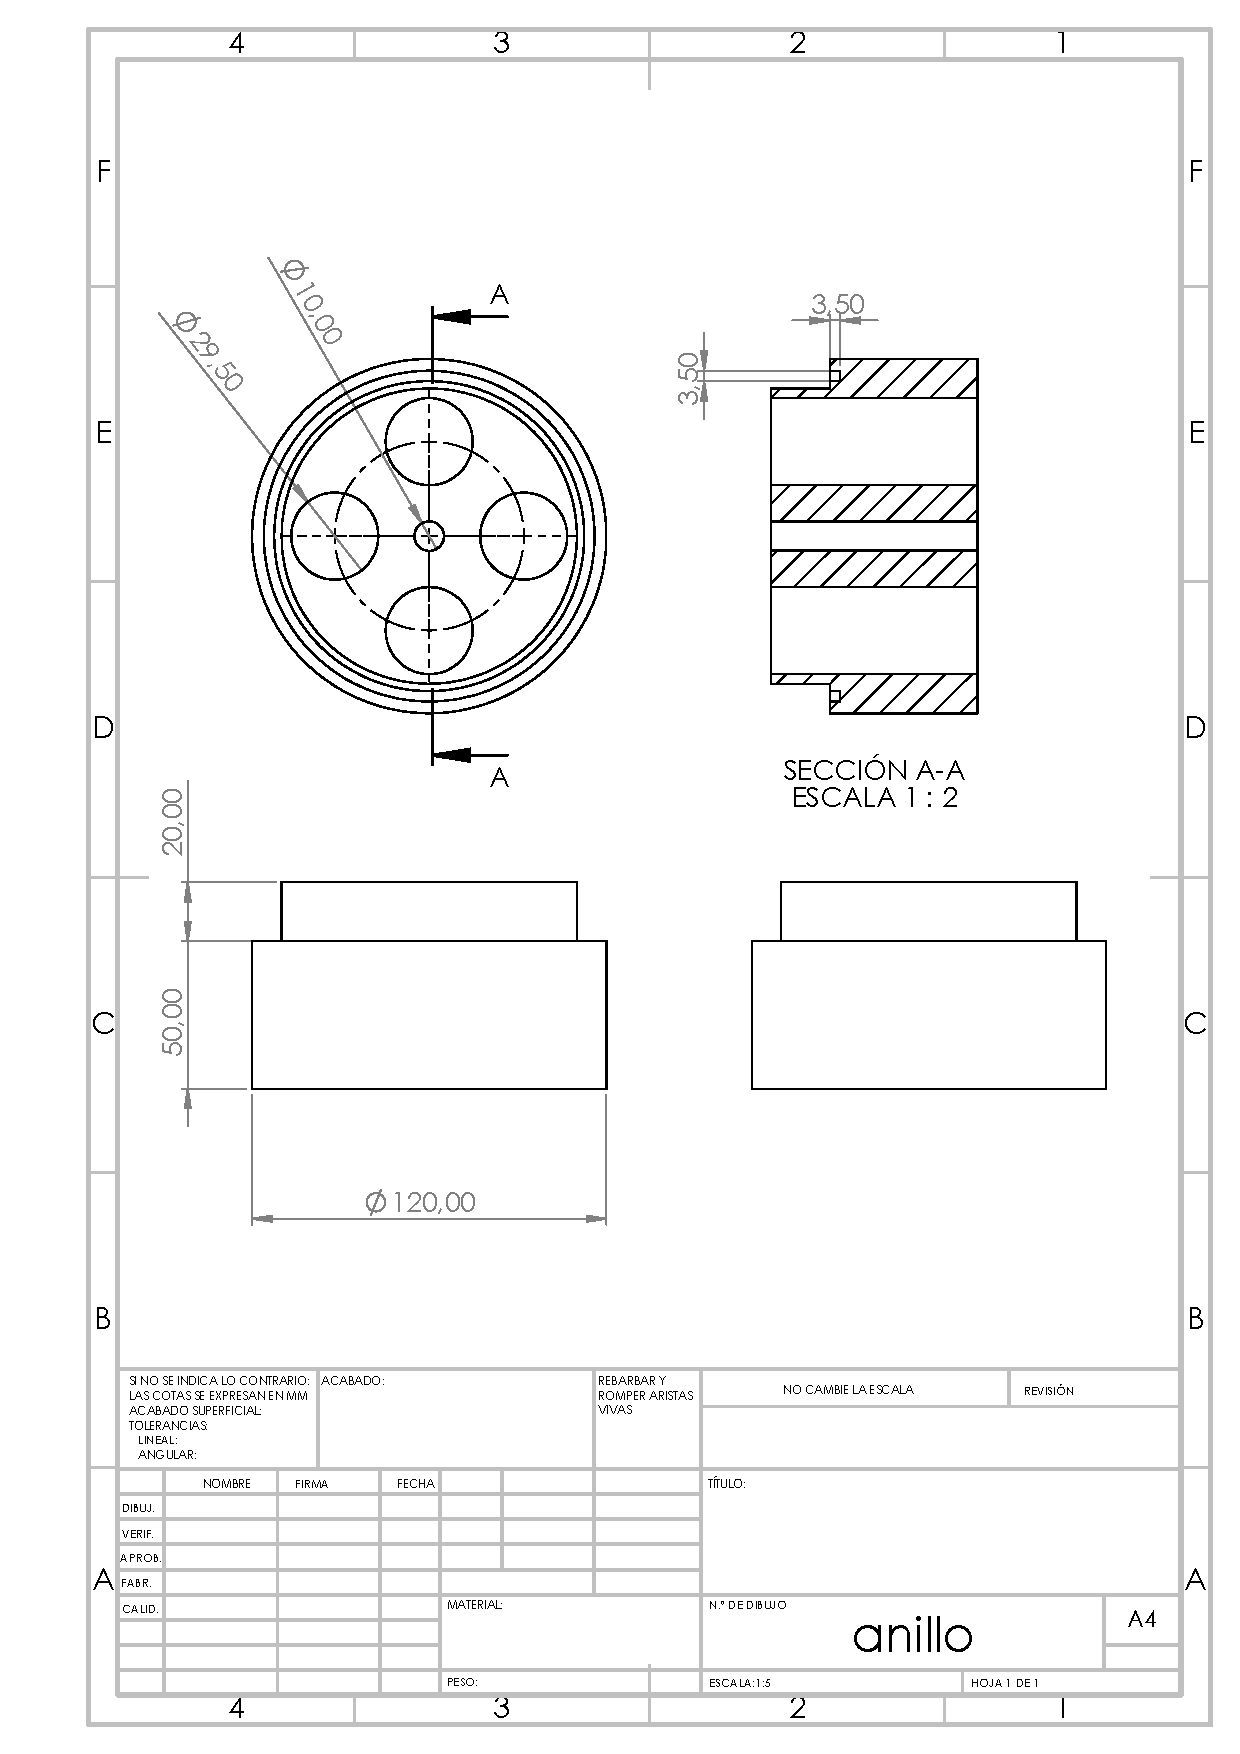
\includegraphics[scale=0.35]{Imagenes/2019/anillo2019.PDF} }
\caption{Dise\~no final del anillo. Fuente: elaboración propia}
\label{fig:Anillo2019}
\end{figure}


\section{Fabricaci\'on}
La fabricación se realizo en el laboratorio de Metal Mec\'anica de la Facultad de Ingenier\'ia Universidad Nacional de Asunción, con un torno semiatom\'atico, con la t\'ecncia de vaciado progresivo. 
 
\begin{figure}[h]
\centering
\fbox{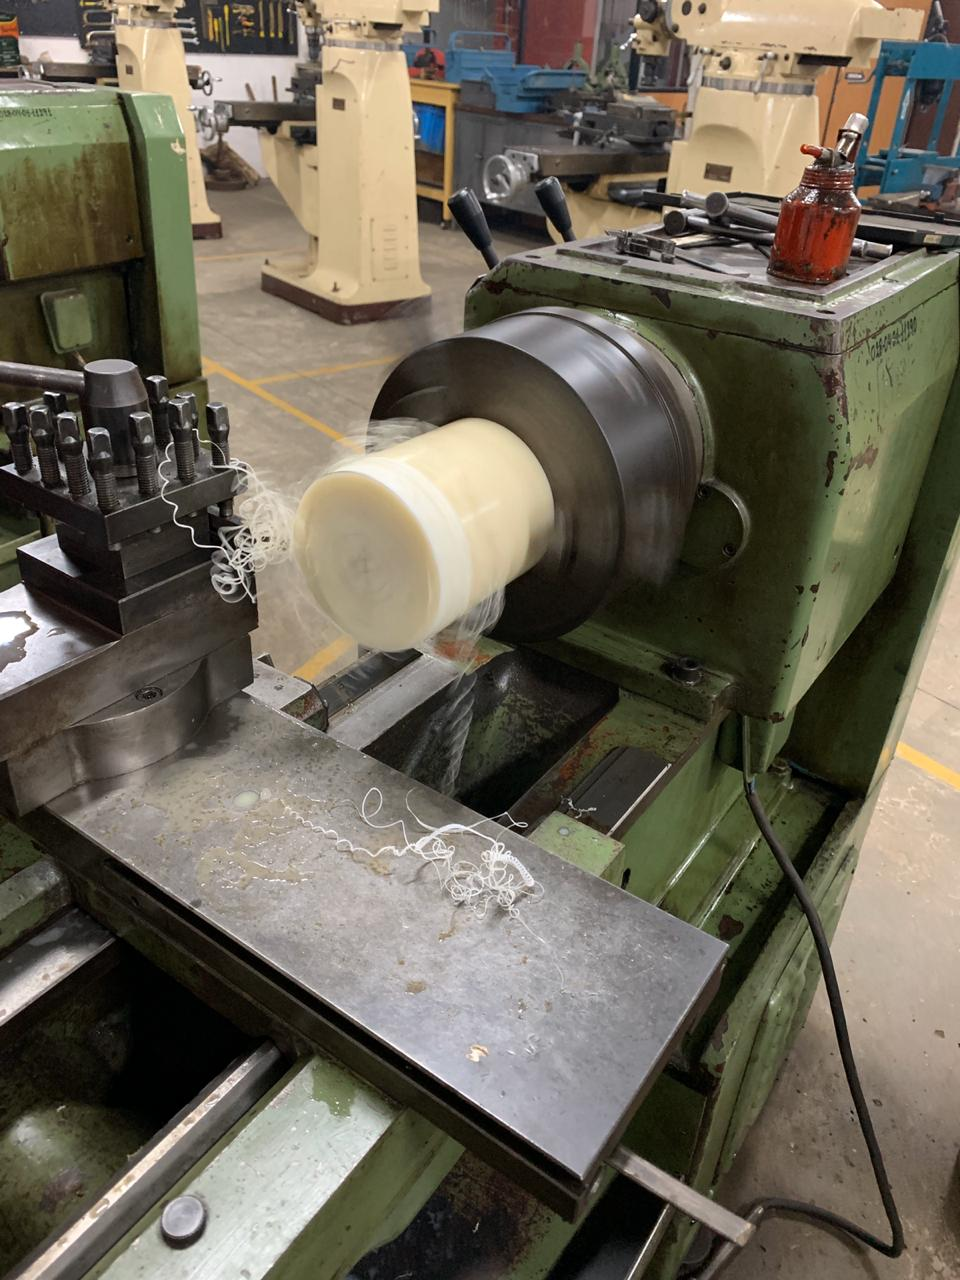
\includegraphics[scale=0.2]{Imagenes/2019/Sonda_Fab0.jpeg} }
\caption{Tubo de Nylon r\'igido en proceso de desgaste. Fuente: elaboración propia}
\label{fig:preparacion}
\end{figure}
 
\hfill
\begin{figure}[t]
\centering
\fbox{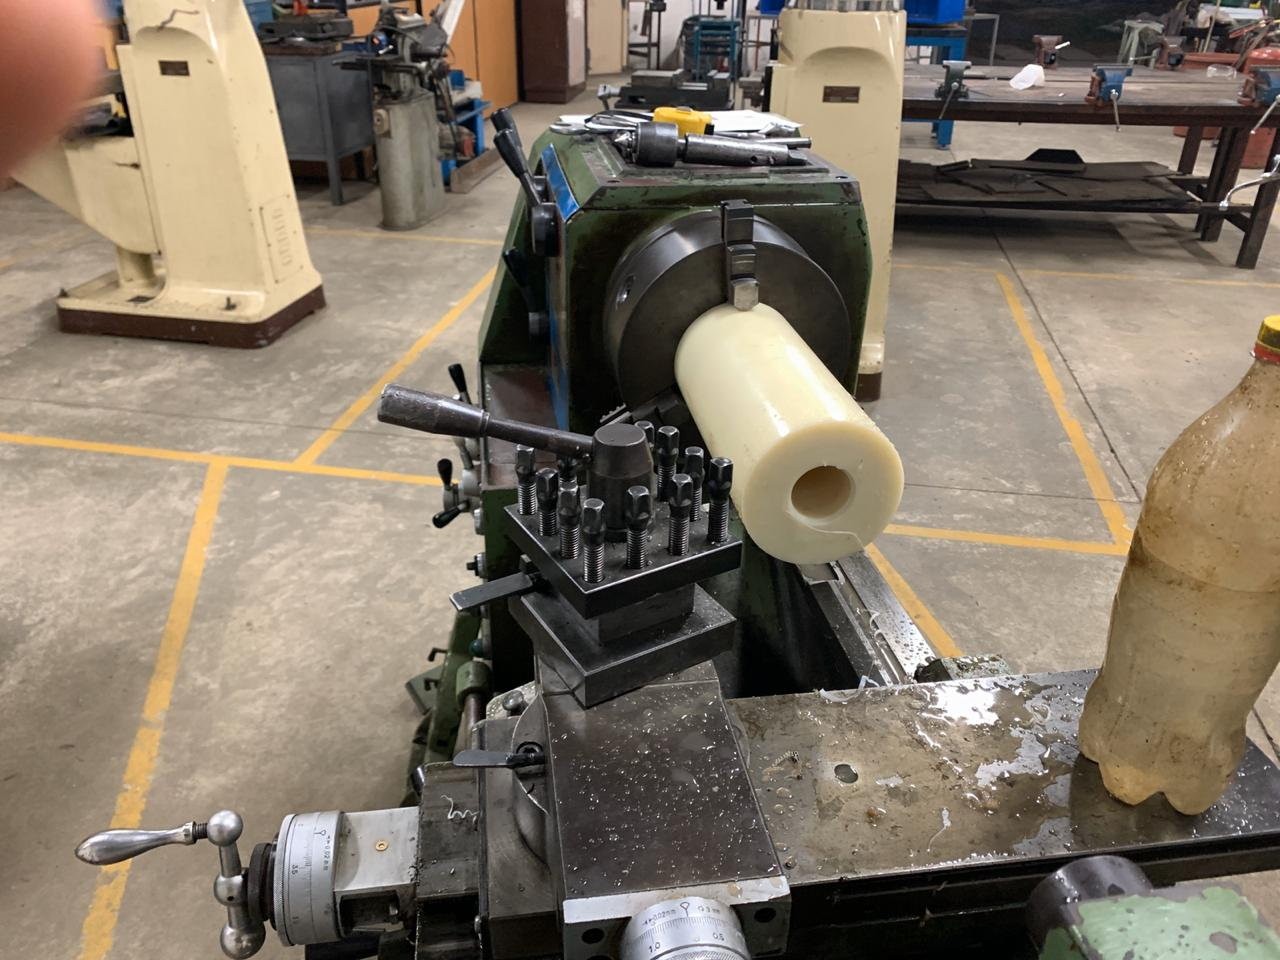
\includegraphics[scale=0.2]{Imagenes/2019/Sonda_Fab.jpeg}}
\caption{Tubo de Nylon r\'igido, proceso de vaciado. Fuente: elaboración propia}
\label{fig:preparacion}
\end{figure}

\section{Programaci\'on e Integraci\'on de los sensores.}
La programa
\section{Almacenamiento y visualizaci\'on de las mediciones.}



%-----------------------------------------------------------------------------